\documentclass[11pt]{article}
\usepackage[utf8]{inputenc}
\usepackage[margin=0.75in]{geometry}
\usepackage{amsmath,amssymb}
\usepackage{chemfig}
\usepackage{chemformula}
\usepackage{tikz}
\usepackage{pgfplots}
\pgfplotsset{compat=1.18}
\usepackage{enumitem}
\usepackage{titlesec}
\usepackage{fancyhdr}

\pagestyle{fancy}
\fancyhf{}
\rhead{USNCO ID Number: \underline{\hspace{3cm}}}
\lhead{2024 U.S. National Chemistry Olympiad National Exam Part II}
\cfoot{\thepage}

\titleformat{\section}{\large\bfseries}{Question \thesection}{1em}{}
\titleformat{\subsection}[runin]{\bfseries}{}{0pt}{}

\begin{document}

\section{1 [10\%]}
An unknown salt $\ch{MX2}$ is a group 2 metal halide.

\subsection*{a.} $10.00\,\text{g}$ $\ch{MX2}$ dissolves in $50.0\,\text{g}$ water to give a homogeneous solution. The freezing point of this solution is $-4.50\text{ }^{\circ}\text{C}$. What is the molar mass of $\ch{MX2}$? For water, $K_f = 1.86\text{ }^{\circ}\text{C}/m$.
\vspace{4cm}

\subsection*{b.} $10.00\,\text{g}$ $\ch{Na2CO3}$ and $10.00\,\text{g}$ $\ch{MX2}$ are mixed in $200.0\,\text{mL}$ of water. A precipitate of $\ch{MCO3}$ forms. What is the pH of the supernatant? The $K_a$ of $\ch{H2CO3}$ is $4.3\times10^{-7}$ and the $K_a$ of $\ch{HCO3-}$ is $4.7\times10^{-11}$.
\vspace{4cm}

\subsection*{c.} A solution of $10.00\,\text{g}$ $\ch{MX2}$ in water is treated with excess silver nitrate. The precipitate is dried; the mass of the dried compound is $15.2\,\text{g}$. What is the identity of $\ch{MX2}$?
\vspace{3cm}

\newpage
\subsection*{d.} A sample of $10.00\,\text{g}$ $\ch{MX2}$ dissolved in $50\,\text{mL}$ water is treated with increasing amounts of $\ch{Na2SO4}$ up to $10\,\text{g}$ in total. How will the mass of precipitate formed vary with the mass of added $\ch{Na2SO4}$? Graph your answer on the grid provided.

\begin{center}
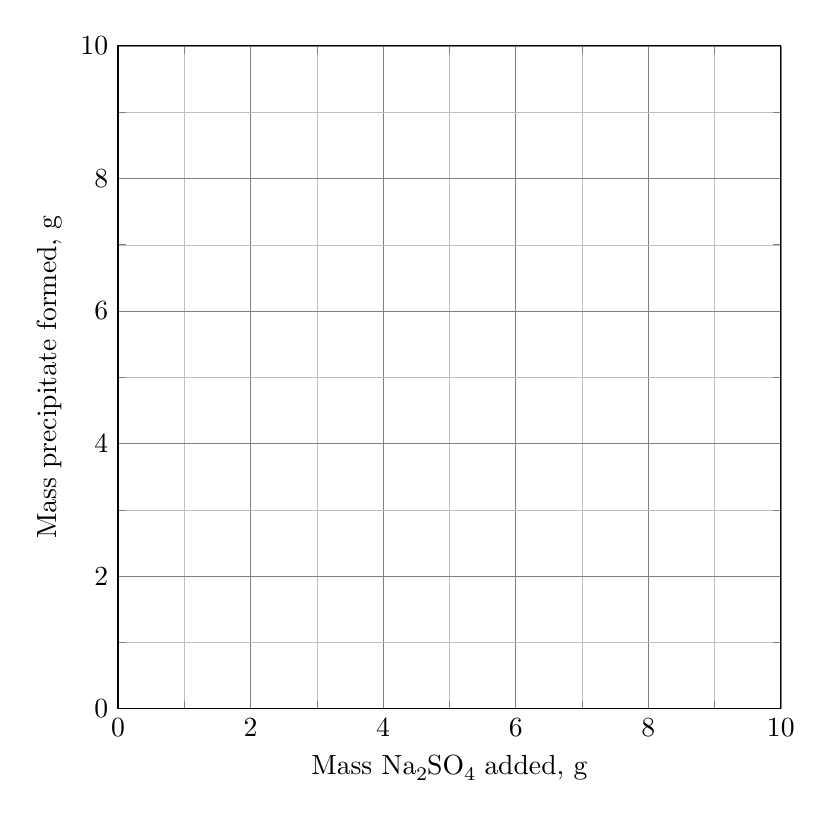
\begin{tikzpicture}
\begin{axis}[
    xmin=0, xmax=10,
    ymin=0, ymax=10,
    xtick={0,2,4,6,8,10},
    ytick={0,2,4,6,8,10},
    grid=both,
    grid style={line width=.1pt, draw=gray!50},
    major grid style={line width=.2pt,draw=gray},
    minor tick num=1,
    xlabel={Mass $\ch{Na2SO4}$ added, g},
    ylabel={Mass precipitate formed, g},
    width=10cm, height=10cm
]
\end{axis}
\end{tikzpicture}
\end{center}

\subsection*{e.} What color flame test does $\ch{MX2}$ give?
\vspace{1.5cm}

\newpage
\section{2 [13\%]}
A sample of solid calcium fluoride is suspended in water in an unreactive container and stirred until it achieves equilibrium. The pH of the solution is lowered by careful addition of nitric acid, and the pH and concentration of $\ch{Ca^{2+}}(aq)$ are noted at several points as shown on the graph below. Note that the units on the y axis are millimoles per liter.

\begin{center}
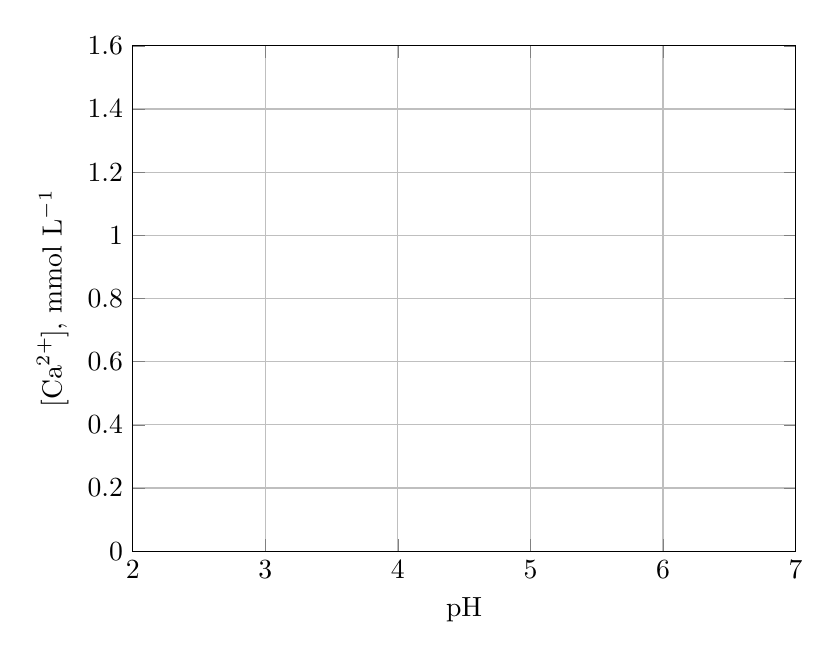
\begin{tikzpicture}
\begin{axis}[
    xmin=2, xmax=7,
    ymin=0, ymax=1.6,
    xtick={2,3,4,5,6,7},
    ytick={0.0,0.2,0.4,0.6,0.8,1.0,1.2,1.4,1.6},
    grid=both,
    xlabel={pH},
    ylabel={$[\ch{Ca^{2+}}]$, mmol L$^{-1}$},
    width=10cm, height=8cm
]
\end{axis}
\end{tikzpicture}
\end{center}

\subsection*{a.} Determine the $K_{sp}$ of $\ch{CaF2}$ from the data provided.
\vspace{3cm}

\subsection*{b.} Qualitatively, what is the cause for the increase in solubility of $\ch{CaF2}$ at low pH?
\vspace{3cm}

\subsection*{c.} From the data provided, determine the $K_a$ of \ch{HF}.
\vspace{3cm}

\subsection*{d.} How many moles of $\ch{HNO3}$ must be added to the $\ch{CaF2}$/water mixture to achieve a $\text{pH} = 3.00$ in this experiment? The volume of solution is $1.00\,\text{L}$.
\vspace{3cm}

\subsection*{e.} Carbon dioxide dissolves in water at $25\text{ }^{\circ}\text{C}$ and $1\,\text{atm}$ pressure to the extent of $0.0345\,\text{mol L}^{-1}$. An aliquot of the solution taken from the above experiment at $\text{pH} = 5$ is stirred under $1\,\text{atm}$ $\ch{CO2}$ and the pH slowly raised by addition of solid $\ch{NaOH}$ until $\ch{CaCO3}$ just begins to precipitate. What is the pH of the solution at this point? The $K_{sp}$ of $\ch{CaCO3}$ is $8.7\times10^{-9}$, the $K_a$ of aqueous $\ch{CO2}$ ("\ch{H2CO3}") is $4.3\times10^{-7}$, and the $K_a$ of $\ch{HCO3-}$ is $4.7\times10^{-11}$.
\vspace{4cm}

\newpage
\section{3 [13\%]}
Ethene, $\ch{C2H4}$, can react in the gas phase in the presence of radicals $\cdot\ch{R}$ to form polyethylene. The forward reaction is second-order while the reverse reaction is first-order.
$$\ch{C2H4}(g) + \cdot\ch{CH2(CH2)_{2n}CH2R} \ch{<=>[k_f][k_r]} \cdot\ch{CH2(CH2)_{2n+2}CH2R}$$

\subsection*{a.} A sample of polyethylene has an average degree of polymerization $n = 1200$. How many polymer chains are present in $1.0\,\text{g}$ of this material?
\vspace{3cm}

\subsection*{b.} Calculate $\Delta H^{\circ}$ and $\Delta S^{\circ}$ for the polymerization reaction from the data:
$$\ln(k_r) = -14500(1/T) + 31.7 \quad (s^{-1})$$
$$\ln(k_f) = -4010(1/T) + 15.2 \quad (\text{bar}^{-1}\text{s}^{-1})$$
\vspace{4cm}

\subsection*{c.} The bond dissociation enthalpy (BDE) for a typical carbon-carbon single bond is $345\,\text{kJ mol}^{-1}$. From the data given, what is the BDE of the carbon-carbon double bond in ethene?
\vspace{3cm}

\subsection*{d.} Ethene is charged to a fixed vessel at $25\,\text{bar}$ and $720\,\text{K}$. Traces of radical are then added to initiate polymerization. What is the percent conversion of ethene into polymer at equilibrium under these conditions?
\vspace{4cm}

\subsection*{e.} In the presence of a catalyst for the polymerization reaction, the forward rate constant as a function of temperature is $\ln(k_f) = -3050(1/T) + 21.0$. By what factor does the catalyst accelerate the rate of the forward reaction at $500\,\text{K}$?
\vspace{3cm}

\subsection*{f.} By what factor does the catalyst change the rate of the reverse reaction at $500\,\text{K}$?
\vspace{2cm}

\newpage
\section{4 [13\%]}
Copper(II) forms a complex ion with ammonia, $\ch{Cu(NH3)4^{2+}}$, with $K_f = 1.7\times10^{13}$. An electrochemical cell is set up at $298\,\text{K}$. Half-cell A contains $100\,\text{mL}$ of $1.00\,\text{M}$ $\ch{Cu(NO3)2}$ while half-cell B contains $100\,\text{mL}$ of a solution that contains a small amount of copper(II) and is $0.100\,\text{M}$ in $\ch{NH3}$. Nitric acid is slowly added to half-cell B and the potential $E$ is recorded.

\subsection*{a.} Which half-cell is the cathode and which is the anode? Justify your answer.
\vspace{3cm}

\subsection*{b.} Qualitatively explain the shape of the titration curve (potential drops slowly, then plummets at the endpoint, and plateaus).
\vspace{3cm}

\subsection*{c.} What is the total concentration of copper(II) in the solution in half-cell B if the plateau potential after the endpoint is $0.14\,\text{V}$?
\vspace{3cm}

\subsection*{d.} If the endpoint occurs at $3.15\,\text{mL}$ of added $\ch{HNO3}$, what is the concentration of nitric acid in the buret?
\vspace{3cm}

\subsection*{e.} Suppose that the experiment is set up again with silver metal in place of copper metal and silver(I) ion in place of copper(II) ion ($\ch{Ag(NH3)2+}$, $K_f = 1.7\times10^7$). Sketch the expected curve on a grid and explain.
\vspace{4cm}

\newpage
\section{5 [12\%]}
Write net equations for each of the reactions below. Omit spectator ions. Show organic structures.
\begin{enumerate}[label=\alph*.]
    \item Aqueous ammonia and acetic acid are mixed.
    \vspace{1.5cm}
    \item Sodium iodate is added to an excess of hydriodic acid.
    \vspace{1.5cm}
    \item Manganese(IV) oxide is added to concentrated aqueous hydrochloric acid.
    \vspace{1.5cm}
    \item Propyl benzoate is heated with aqueous sodium hydroxide.
    \vspace{1.5cm}
    \item Calcium oxide and graphite are heated to $2200\text{ }^{\circ}\text{C}$.
    \vspace{1.5cm}
    \item Iodine-124 undergoes radioactive decay by electron capture.
    \vspace{1.5cm}
\end{enumerate}

\newpage
\section{6 [14\%]}
Consider the properties of the group 1 elements in the table below:
\begin{center}
\begin{tabular}{|c|c|c|c|}
\hline
Element & First IE ($\text{kJ mol}^{-1}$) & Excite to $(n+1)s$ ($\text{kJ mol}^{-1}$) & Density of $\ch{MCl(s)}$ ($\text{mol cm}^{-3}$)\\
\hline
H & 1312 & 984 & 0.0403 \\
Li & 520 & 325 & 0.0507 \\
Na & 496 & 308 & 0.0371 \\
K & 420 & 252 & 0.0266 \\
Rb & 403 & 241 & 0.0232 \\
Cs & 376 & 222 & 0.0237 \\
\hline
\end{tabular}
\end{center}

\subsection*{a.} Rationalize the observed trend in first ionization energies with increasing $n$.
\vspace{2cm}

\subsection*{b.} If a hydrogen atom excited to its $2s^1$ state transfers its electron to $\ch{Cs+}$ to form a ground-state Cs atom, how much energy is absorbed or released?
\vspace{2.5cm}

\subsection*{c.} All but one of the atoms have an excited state significantly lower in energy than the $(n+1)s^1$ state. Explain, noting the exception.
\vspace{2.5cm}

\subsection*{d.} All but one of the atoms have an excited state modestly higher in energy ($38-55\,\text{kJ mol}^{-1}$) than the $(n+1)s^1$ state. Explain, noting the exception.
\vspace{2.5cm}

\subsection*{e.} Explain the trend in $\ch{MCl}$ molar densities, and reasons for the exceptions ($\ch{HCl}$ and $\ch{CsCl}$).
\vspace{3cm}

\subsection*{f.} $^{137}\text{Cs}$ ($136.9070895\,\text{amu}$) decays to a stable product ($136.9058274\,\text{amu}$). Identify the decay mode and product.
\vspace{2cm}

\subsection*{g.} Calculate the energy released in $\text{kJ mol}^{-1}$ by this decay.
\vspace{2cm}

\newpage
\section{7 [13\%]}
Flash vacuum pyrolysis of carbonyl azide ($\ch{CON6}$) at $420\text{ }^{\circ}\text{C}$ gives diazirinone.

\subsection*{a.} Draw complete Lewis structures for carbonyl azide and diazirinone.
\vspace{4cm}

\subsection*{b.} Diazirinone decomposes to $\ch{CO}(g)$ and $\ch{N2}(g)$. Estimate $\Delta H^{\circ}$ using the given BDEs:
$\text{C-O}=350$, $\text{C=O}=741$, $\ch{C\#O}=1080$, $\text{C-N}=290$, $\text{C=N}=615$, $\ch{C\#N}=891$, $\text{N-N}=160$, $\text{N=N}=418$, $\ch{N\#N}=949\,\text{kJ mol}^{-1}$.
\vspace{3cm}

\subsection*{c.} The actual $\Delta H^{\circ}$ is $-347\,\text{kJ mol}^{-1}$. Comment on the discrepancy.
\vspace{2.5cm}

\subsection*{d.} Will $\Delta G^{\circ}$ at $298\,\text{K}$ be greater than, less than, or equal to $\Delta H^{\circ}$?
\vspace{2cm}

\subsection*{e.} An acyclic isomer has the connectivity NCNO. Draw its Lewis structure and describe its geometry.
\vspace{3cm}

\subsection*{f.} Predict whether acyclic NCNO is more or less stable than diazirinone.
\vspace{2.5cm}

\newpage
\section{8 [12\%]}
Consider isomers I, II, and III of $\ch{C4H9NO2}$:
\begin{center}
\begin{enumerate}[label=\Roman*.]
\item \chemfig{CH_3O-CH_2-CH_2-C(=O)-NH_2} \\
\item \chemfig{H_2N-CH_2-CH_2-C(=O)-OCH_3} \\
\item \chemfig{HO-CH_2-CH_2-CH_2-CH=N-OH}
\end{enumerate}
\end{center}

\subsection*{a.} Which compound is the most basic? Justify your answer.
\vspace{2.5cm}

\subsection*{b.} Draw the structures of the conjugate acids of all three.
\vspace{3cm}

\subsection*{c.} Draw the structure of a chiral isomer of $\ch{C4H9NO2}$.
\vspace{2.5cm}

\subsection*{d.} Consider N-methylpyrrole (IV) and N-methylimidazole (V):
\begin{center}
\begin{enumerate}[label=\Roman*., start=4]
\item \chemfig{*5(-N(CH_3)-=-=-)} \\
\item \chemfig{*5(-N(CH_3)-=N-=-)}
\end{enumerate}
\end{center}
Which compound is more basic? Draw its conjugate acid structure.
\vspace{3cm}

\subsection*{e.} Which compound is more reactive towards $\ch{Br2}$? Explain and draw the major product.
\vspace{4cm}

\newpage
\begin{center}
{\Large \textbf{2024 USNCO Part II SOLUTIONS / ANSWER KEY}}
\end{center}
\setcounter{section}{0}

\section{1 Solutions}
\begin{enumerate}[label=\alph*.]
    \item $m = \frac{4.50}{1.86} = 2.42\,\text{m}$. Since $\ch{MX2} \rightarrow \ch{M^{2+}} + \ch{2X-}$, $i=3$.
    $m_{\text{salt}} = \frac{2.42}{3} = 0.807\,\text{m}$.
    $\text{Moles} = 0.807 \times 0.0500\,\text{kg} = 0.0404\,\text{mol}$.
    $M = \frac{10.00\,\text{g}}{0.0404\,\text{mol}} = 248\,\text{g mol}^{-1}$.
    \item $\text{Mol }\ch{Na2CO3} = \frac{10.00}{105.99} = 0.0944\,\text{mol}$. Residual $\ch{CO3^{2-}} = 0.0944 - 0.0404 = 0.0540\,\text{mol}$.
    $[\ch{CO3^{2-}}] = \frac{0.0540}{0.200} = 0.270\,\text{M}$.
    $K_b = \frac{K_w}{K_{a2}} = \frac{1.0\times10^{-14}}{4.7\times10^{-11}} = 2.13\times10^{-4}$.
    $[\ch{OH-}] = \sqrt{2.13\times10^{-4} \times 0.270} = 7.6\times10^{-3}\,\text{M} \implies \text{pH} = 11.88$.
    \item $\text{Mol }\ch{X-} = 2 \times 0.0404 = 0.0808\,\text{mol}$. Molar mass of $\ch{AgX} = \frac{15.2}{0.0808} = 188\,\text{g mol}^{-1} \implies \ch{X} = \ch{Br}$.
    $M_{\ch{M}} = 248 - 2(79.9) = 88.2\,\text{g mol}^{-1} \implies \ch{M} = \ch{Sr}$. Formula: $\ch{SrBr2}$.
    \item Max mass of $\ch{SrSO4} = 0.0404\,\text{mol} \times 183.68\,\text{g mol}^{-1} = 7.42\,\text{g}$. Equivalent mass of $\ch{Na2SO4} = 0.0404 \times 142.04 = 5.74\,\text{g}$. The plot rises linearly from $(0,0)$ to $(5.74, 7.42)$ and then plateaus.
    \item Strontium gives a \textbf{red} flame test.
\end{enumerate}

\section{2 Solutions}
\begin{enumerate}[label=\alph*.]
    \item At high pH, solubility $\approx 0.21\,\text{mmol L}^{-1} = 2.1\times10^{-4}\,\text{M}$.
    $K_{sp} = [\ch{Ca^{2+}}][\ch{F-}]^2 = (2.1\times10^{-4})(4.2\times10^{-4})^2 = 3.7\times10^{-11}$.
    \item $\ch{F-}$ is protonated by $\ch{H+}$ to form $\ch{HF}$, depleting free $[\ch{F-}]$ and shifting the dissolution equilibrium forward via Le Chatelier's principle.
    \item At $\text{pH}=2$, $[\ch{Ca^{2+}}] = 1.36\times10^{-3}\,\text{M}$. Total $[\ch{F}]_{\text{tot}} = 2.72\times10^{-3}\,\text{M}$.
    $[\ch{F-}] = \sqrt{\frac{3.7\times10^{-11}}{1.36\times10^{-3}}} = 1.65\times10^{-4}\,\text{M}$.
    $[\ch{HF}] = 2.72\times10^{-3} - 1.65\times10^{-4} = 2.56\times10^{-3}\,\text{M}$.
    $K_a = \frac{(10^{-2})(1.65\times10^{-4})}{2.56\times10^{-3}} = 6.4\times10^{-4}$.
    \item At $\text{pH}=3$, $[\ch{Ca^{2+}}] = 3.9\times10^{-4}\,\text{M} \implies [\ch{F}]_{\text{tot}} = 7.8\times10^{-4}\,\text{M}$.
    $\frac{[\ch{F-}]}{[\ch{HF}]} = \frac{6.4\times10^{-4}}{10^{-3}} = 0.64 \implies [\ch{HF}] = 4.8\times10^{-4}\,\text{M}$.
    $\text{Mol }\ch{HNO3} = [\ch{HF}] + [\ch{H+}] = 4.8\times10^{-4} + 1.0\times10^{-3} = 1.5\times10^{-3}\,\text{mol}$.
    \item $[\ch{Ca^{2+}}] = 2.1\times10^{-4}\,\text{M} \implies [\ch{CO3^{2-}}] = \frac{8.7\times10^{-9}}{2.1\times10^{-4}} = 4.14\times10^{-5}\,\text{M}$.
    $\frac{[\ch{CO3^{2-}}][\ch{H+}]^2}{[\ch{H2CO3}]} = K_{a1}K_{a2} = 2.02\times10^{-17} \implies [\ch{H+}] = 1.3\times10^{-7}\,\text{M} \implies \text{pH} = 6.88$.
\end{enumerate}

\section{3 Solutions}
\begin{enumerate}[label=\alph*.]
    \item $M = 1200 \times 28.05 = 33660\,\text{g mol}^{-1}$. Chains in $1.0\,\text{g} = \frac{1.0}{33660} \times N_A = 1.8\times10^{19}$.
    \item $\ln(K_{eq}) = \ln(k_f) - \ln(k_r) = 10490(1/T) - 16.5$.
    $\Delta H^{\circ} = -10490 \times R = -87.2\,\text{kJ mol}^{-1}$. $\Delta S^{\circ} = -16.5 \times R = -137\,\text{J mol}^{-1}\text{K}^{-1}$.
    \item $\Delta H^{\circ} = \text{BDE}(\ch{C=C}) - 2\,\text{BDE}(\text{C-C}) \implies -87.2 = \text{BDE}(\ch{C=C}) - 2(345) \implies \text{BDE}(\ch{C=C}) = 603\,\text{kJ mol}^{-1}$.
    \item At $720\,\text{K}$, $K_p = e^{10490/720 - 16.5} = 0.145\,\text{bar}^{-1}$. $P_{\ch{C2H4}} = 1/K_p = 6.9\,\text{bar}$.
    $\% \text{ conversion} = \frac{25 - 6.9}{25} \times 100\% = 72.4\%$.
    \item At $500\,\text{K}$, $\frac{k_{\text{cat}}}{k_{\text{uncat}}} = \frac{e^{-3050/500 + 21.0}}{e^{-4010/500 + 15.2}} = \frac{1.32\times10^6}{584} = 2260$.
    \item A catalyst does not change $K_{eq}$, so the reverse reaction rate increases by the identical factor of $2260$.
\end{enumerate}

\section{4 Solutions}
\begin{enumerate}[label=\alph*.]
    \item Half-cell A has higher $[\ch{Cu^{2+}}]$ ($1.00\,\text{M}$) than cell B where copper is complexed. Reduction occurs spontaneously at higher concentration $\implies$ Half-cell A is the \textbf{cathode}, B is the \textbf{anode}.
    \item Initial addition of $\ch{HNO3}$ buffers the free ammonia concentration, giving a slow change in cell potential. Near the equivalence point, free ammonia drops rapidly, causing free $[\ch{Cu^{2+}}]$ to shoot up and the potential to plummet. Past the endpoint, all ammonia is protonated, leaving free aquated $\ch{Cu^{2+}}$ at a constant concentration, causing the potential to plateau.
    \item Past the endpoint, $0.14 = 0 - \frac{0.0592}{2}\log\left(\frac{[\ch{Cu^{2+}}]_B}{1.00}\right) \implies [\ch{Cu^{2+}}]_B = 1.8\times10^{-5}\,\text{M}$.
    \item $\text{Moles of }\ch{NH3} = 0.100\,\text{L} \times 0.100\,\text{M} = 0.0100\,\text{mol}$. $[\ch{HNO3}] = \frac{0.0100\,\text{mol}}{0.00315\,\text{L}} = 3.17\,\text{M}$.
    \item Before the endpoint, because $n=1$ for $\ch{Ag+}$, the slope factor $\frac{RT}{F}$ vs $\frac{RT}{2F}$ changes, shifting potentials up by $\approx 0.18\,\text{V}$. After the endpoint, the absence of the $\frac{1}{2}$ factor doubles the cell potential step to $\approx 0.28\,\text{V}$.
\end{enumerate}

\section{5 Solutions}
\begin{enumerate}[label=\alph*.]
    \item $\ch{NH3} + \ch{CH3COOH} \rightarrow \ch{NH4+} + \ch{CH3COO-}$
    \item $\ch{IO3-} + \ch{8I-} + \ch{6H+} \rightarrow \ch{3I3-} + \ch{3H2O}$ (or forming $\ch{I2}$)
    \item $\ch{MnO2} + \ch{4H+} + \ch{2Cl-} \rightarrow \ch{Mn^{2+}} + \ch{Cl2} + \ch{2H2O}$
    \item \chemfig{*6(-=-=-(-C(=O)-O-CH_2-CH_2-CH_3)=)} $+ \ch{OH-} \rightarrow$ \chemfig{*6(-=-=-(-C(=O)-O^-)=)} $+ \ch{CH3CH2CH2OH}$
    \item $\ch{CaO} + \ch{3C} \rightarrow \ch{CaC2} + \ch{CO}$
    \item $\ch{^{124}_{53}I} + \ch{^0_{-1}e} \rightarrow \ch{^{124}_{52}Te}$
\end{enumerate}

\section{6 Solutions}
\begin{enumerate}[label=\alph*.]
    \item As $n$ increases, the valence shell is further from the nucleus. Since $Z_{\text{eff}}$ remains roughly constant, the Coulombic attraction decreases, lowering the ionization energy.
    \item $E_{2s}(\ch{H}) = -1312 + 984 = -328\,\text{kJ mol}^{-1}$. $\ch{Cs}$ valence ground state is $-376\,\text{kJ mol}^{-1}$. $\Delta E = -376 - (-328) = -48\,\text{kJ mol}^{-1}$ (releases $48\,\text{kJ mol}^{-1}$).
    \item For $\ch{Li}$ to $\ch{Cs}$, promotion to the $np$ orbital is available and lower in energy than $(n+1)s$. \textbf{H} is the exception because there is no $1p$ subshell.
    \item The $(n+1)p$ orbital is slightly higher than $(n+1)s$ for multi-electron atoms due to shielding differences. \textbf{H} is the exception because subshell energies depend purely on $n$ for single-electron systems ($2s$ and $2p$ are degenerate).
    \item $\ch{LiCl}$ through $\ch{RbCl}$ form rock-salt ionic lattices; larger cations increase lattice spacing, decreasing density. \textbf{\ch{HCl}} forms weak molecular crystals with wider spacing (less dense). \textbf{\ch{CsCl}} switches to a primitive cubic packing with a higher coordination number ($8:8$), making it more densely packed.
    \item $\beta^-$ decay forming $^{137}\text{Ba}$.
    \item $\Delta m = 136.9070895 - 136.9058274 = 0.0012621\,\text{amu} = 2.096\times10^{-30}\,\text{kg}$. $E = \Delta m c^2 \times N_A = 1.13\times10^8\,\text{kJ mol}^{-1}$.
\end{enumerate}

\section{7 Solutions}
\begin{enumerate}[label=\alph*.]
    \item Carbonyl Azide: \chemfig{O=C(-N=\overset{+}{N}=\overset{-}{N})_2} \qquad Diazirinone: \chemfig{O=C*3(-N=N-)}
    \item $\Delta H^{\circ} = [\text{BDE}(\ch{C=O}) + \text{BDE}(\ch{N=N}) + 2\,\text{BDE}(\text{C-N})] - [\text{BDE}(\ch{C\#O}) + \text{BDE}(\ch{N\#N})] = [741 + 418 + 2(290)] - [1080 + 949] = -290\,\text{kJ mol}^{-1}$.
    \item Discrepancy due to severe \textbf{ring strain} in the 3-membered ring of diazirinone, making reactant bonds weaker and the overall decomposition more exothermic than predicted by average BDEs.
    \item $\Delta G^{\circ} < \Delta H^{\circ}$ because $\Delta S^{\circ} > 0$ ($1 \text{ molecule} \rightarrow 2 \text{ gas molecules}$).
    \item $\ch{N\#C-N=O}$. Linear at carbon, bent ($\approx 120^\circ$) at the internal nitrogen.
    \item Diazirinone is expected to be more stable because acyclic NCNO contains less stable individual bonds ($\ch{C=N}$, $\ch{N=O}$) compared to the strong $\ch{C=O}$ double bond retained in diazirinone.
\end{enumerate}

\section{8 Solutions}
\begin{enumerate}[label=\alph*.]
    \item \textbf{II} is most basic. Its nitrogen lone pair resides on an $sp^3$ amine, whereas in I the lone pair is deactivated by resonance with the carbonyl group (amide), and in III the lone pair is on a less basic $sp^2$ oxime nitrogen bonded to an electronegative oxygen.
    \item Conjugate acids:
    I: \chemfig{CH_3O-CH_2-CH_2-C(\overset{+}{O}H)-NH_2} \quad
    II: \chemfig{H_3\overset{+}{N}-CH_2-CH_2-C(=O)-OCH_3} \quad
    III: \chemfig{HO-CH_2-CH_2-CH_2-CH=\overset{+}{N}(H)-OH}
    \item Chiral isomer: \chemfig{CH_3-CH(NH_2)-C(=O)-OCH_3}
    \item \textbf{V (N-methylimidazole)} is more basic. Protonation occurs at the $sp^2$ pyridine-like nitrogen, maintaining aromaticity and establishing symmetrical resonance stabilization of the positive charge over both nitrogens. Pyrrole (IV) loses aromaticity upon protonation on nitrogen.
    \item \textbf{IV (N-methylpyrrole)} is more reactive. Its lone pair directly participates in the $\pi$-system, making the carbons highly nucleophilic. In V, the second nitrogen is electron-withdrawing. Major product: \chemfig{*5(-N(CH_3)-=(\alpha-Br)-=-)} (bromination at the 2-position).
\end{enumerate}

\end{document}